\documentclass[10pt,twocolumn,letterpaper]{article}

\usepackage{cvpr}
\usepackage{times}
\usepackage{epsfig}
\usepackage{graphicx}
\usepackage{amsmath}
\usepackage{amssymb}
\usepackage{algorithm2e}

% Include other packages here, before hyperref.

% If you comment hyperref and then uncomment it, you should delete
% egpaper.aux before re-running latex.  (Or just hit 'q' on the first latex
% run, let it finish, and you should be clear).
\usepackage[breaklinks=true,bookmarks=false]{hyperref}
\newcommand*\samethanks[1][\value{footnote}]{\footnotemark[#1]}

\cvprfinalcopy % *** Uncomment this line for the final submission

\def\httilde{\mbox{\tt\raisebox{-.5ex}{\symbol{126}}}}

% Pages are numbered in submission mode, and unnumbered in camera-ready
%\ifcvprfinal\pagestyle{empty}\fi
\setcounter{page}{1}
\begin{document}

%%%%%%%%% TITLE
\title{Generating Slides from HTML pages}

\author{Arun JVS\thanks{IIIT, Hyderabad}\\
201001079\\
{\tt\small arun.jvs\thanks{@students.iiit.ac.in}}
% For a paper whose authors are all at the same institution,
% omit the following lines up until the closing ``}''.
% Additional authors and addresses can be added with ``\and'',
% just like the second author.
% To save space, use either the email address or home page, not both
\and
Rohit Girdhar\samethanks[1]\\
201001047\\
{\tt\small rohit.girdhar\samethanks[2] }
\and
Sudheer Kumar\samethanks[1]\\
201001149\\
{\tt\small sai.shanka\samethanks[2] }
}

\maketitle
%\thispagestyle{empty}

%%%%%%%%% ABSTRACT
\begin{abstract}
    Authors of technical papers often use slides to effectively present their ideas in
conferences and meetings. If there is an easy way of generating slides from a
research paper, then it would be of great use to them. In this paper, we propose the
framework of an automated system which takes the HTML version of a technical paper and generates a starting point presentation with organized headings, images, summarized
text and references that can be further turned into a final presentation. HTML version
of any paper which is in accordance with conference/journal proceedings can be given
as input to out system. The HTML file is parsed, information in it is extracted and is
converted into a predefined XML format. Then the data in this XML file is summarized
using multiple heuristics to generate most informative content. The summarized content
is then converted into a neat \LaTeX\ presentation.
\end{abstract}

%%%%%%%%% BODY TEXT
\section{Motivation}

Presenting information using slides is an effective way for audience retention.
Presenters take the aid of slides for presenting research papers in conferences, for
explaining them in classrooms and for other academic purposes. But creating slides from
the research papers is a time consuming task for the presenter. So, it would be a great
benefit for them if there is an easy way for generating the slides from the research
papers. Also, sometimes people want to go through the research papers just to understand
the overview of them. Slides provide an easier way for them to understand the overview of
the topic. This gives rise to need for a tool which automatically generates slides from
research papers. Automatic generation of slides from research paper is an easier task
compared to generation of slides from some random document because research papers have
an almost similar structure and we can address the problem of automatic generation of slides
from research papers by exploiting the structure of the research papers. Once this problem
is addressed, this work can be easily extended to automatically generate slides from other
structured entities like book chapters etc.

\section{Problem Definition}
Given an HTML version of a research paper which is in accordance with the conference/journal
proceedings, a slideshow is created which contains an summarized version of the paper.
This Slideshow will contain the important points, tables, graphs, figures which helps to
explain the paper. This may not serve as a final presentation but provides a good starting
point for preparing it.

\section{Related Work}
There has been limited work that addresses the problem of automatic slides generation.
Previous works include approaches like section-wise summarization \cite{sravanthi},
alignment methods for matching document regions with presentation regions \cite{brandon},
extracting topics and itemized elaborations from tagged documents.
Many of these systems use multiple ideas from Information Retrieval, such as TF-IDF weights,
query expansion, query-specific summarization, POS-tagging, etc..
Some of them are purely generative, while others learn models from an existing corpus of
document-presentation pairs. These systems are tuned to work with different input formats
such as PDF, XML, \LaTeX\ and PPT, each of which preserve a varying amount of semantic and
structural information about the original text. In the following two subsections, we review
two papers \cite{sravanthi},\cite{brandon} which particularly deal with technical papers.

\subsection{SlidesGen}
The first work we review is by Sravanthi et al. \cite{sravanthi}. They propose an
novel framework for automatic generation of presentation slides for technical papers.
They take \LaTeX\ documents of research papers as input, and return the presentation slides.
Their method depends on the assumption that by and large, conference papers have a similar structure:
an abstract, followed by sections that can be broadly classified as introduction, related work,
actual work (model), experiments, conclusion/results and bibliography.
A slide in their system contains a title and some bulleted points that are important in 
that section. They evaluate the system by surveying the response of people who use their system.

Their system is divided into multiple stages. The first stage is pre-processing stage.
In this step, the \LaTeX\ documents are converted into XML using a public domain converter
LaTeXML. 

Next, the generate what they call "configuration file", which contains configuration
parameters for each section (since each section has a different point of view and writing style).
This involves categorization of the section and extraction of key phrases from the section
which are then stored in the configuration file.
For example, a section with large number of cite tags, or with title containing words such as
"related work" or "literature survey" is categorized as related works section.

The next step is of extracting key phrases.	Most research papers have associated key phrases 
that can be help categorize the content in paper, and contain important concepts introduced
in the paper. They are mostly related to model and experiments section, and can be used to 
summarize the same. So, the keywords given at the beginning are added to keyphrases for those
sections in the configuration file. Also, few other phrases as the names of subsections etc 
are also added to the configuration file.

Next, they use QueSTS summarizer to summarize the model, experiment and conclusions section.
QueSTS represents the text as a Integrated Graph where sentence is a node, and edge exists 
between 2 sentences if the sentences are similar. The edge weight is defined as the 
cosine similarity between the 2 sentences (above a given minimum threshold)
Given the keyphrases computed previously, they are tokenized and 
a centrality based (to the query phrase) node weight is computed for the node corresponding to each token.
Thus, they get query specific node weights and query independent edge weights.

From the above graph, they construct a Contextual Tree for each term $q$ and node $r$.
All the trees at node $r$ are merged into a Summary Graph at $r$. The SGraphs generated
from each node are ranked using a scoring model, and the one with best rank is returned as
the summary.

The final step of this procedure is slide generation from the XML and configuration file.
The introduction slides are generated by comparing introduction sentence with the abstract 
using consine similarity and ones with high similarity are placed in the slides.
They give a similar method for generating slides from related work section as well.
From model and experiments section, the slides are generated using the above QueSTS
mechanism. Similarly, conclusion slides are generated using comparison with keywords
such as "proposed", "concluded" etc.

Another important aspect in slides is graphics. Graphics are added along with sentences 
that either refer to it or is present along with it.

The paper finally discusses the issues in alignment of sentences and generation of slides.
They also evaluate their slides manually with multiple users, taking their feedback.
Most users gave a satisfaction level of more than 8/10 to the slides generated.

\subsection{Alignment Methods}
This paper by Brandon et. al. \cite{brandon} takes a different approach to slide generation,
inspired by the human throught process while making a slide out of a paper.
They focus their efforts on \textit{alignment} methods - first breaking up the document and
presentation into regions and then performing a matching on them.
\textit{Slide regions} include bullets, headings, and other text spans, while \textit{Paper regions}
include paragraphs, section headings, and list items.

They generate their corpus of 296 paper-presentation pairs from workshops of technical conferences,
through simple searching. The papers were PDF format, and presentation were a mixture of PDF and PPT.
Before working with them, they convert them into custom XML formats, which represent relevant parts of
the original data as logical regions (orthographic boundaries). They prefer such physical regions over
semantic regions for its simplicity to implement and verify.

The alignment problem now reduces to an IR query, where the query is a slide region (which is the
section/subsection the slide is related to), and the documents are the target regions from the paper.
They compare two TF-IDF based scoring methods, with and without query expansion, resulting in 4
alignment methods.

The procedure of scoring is as follows. For each token in each region TF-IDF is computed, where TF is
the frequency of the token in the region and DF is the number of regions containing the token's stem.
The slide region is tokenized and POS tagged to remove non-content words. Each token in the query is
stemmed and then may or may not be query-expanded depending on the method. A score is then calculated
for each target region with the query. Two scoring methods were used - one uses the average TF-IDF
score of the search terms relative to the target region, and the other uses the quantity of the matched
terms.

The evaluation of their methods gives critical insights. First, a vast majority of the slide regions are
not alignable (zero score with all target regions) - meaning that a lot of information in slides is not
present in the paper - contrary to their hypothesis. Then they define an \textit{alignable} accuracy against
the \textit{raw} accuracy, considering only alignable slide regions. They find that the best algorithm
on an average gives an average 75\% alignable accuracy, but only 50\% raw accuracy. Query expansion seems
to have little or negative impact on the aligners and that the second scoring method is better than
the first.

After more results, they conclude that the data indicates that the task of presentation generation
is highly dependent on the end purpose the presentation will serve, as well as the target audience and other
factors. Also query expansion generally degraded performance, possibly because authors tend to use wording in
slides similar to their paper, and that using synonyms for query expansion is not aggressive enough, and may
require hypernyms, immediate hyponyms, and other semantically related terms. Also a possible loss of accuracy
could be polysemy of words, causing query expansion to be incorrect and insensitive to context.


%\begin{figure}[t]
%\begin{center}
%\fbox{\rule{0pt}{2in} \rule{0.9\linewidth}{0pt}}
%   %\includegraphics[width=0.8\linewidth]{egfigure.eps}
%\end{center}
%   \caption{Example of caption.  It is set in Roman so that mathematics
%   (always set in Roman: $B \sin A = A \sin B$) may be included without an
%   ugly clash.}
%\label{fig:long}
%\label{fig:onecol}
%\end{figure}

\section{Approach}


\begin{figure*}
\begin{center}
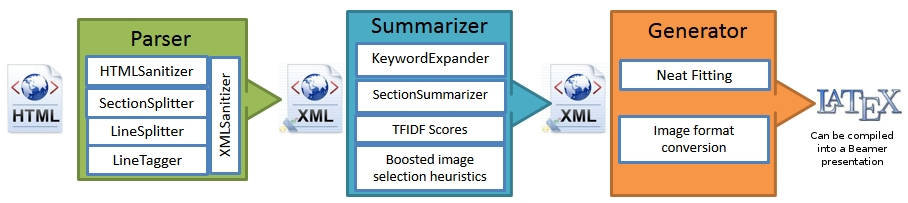
\includegraphics[width=\linewidth]{system.jpg}
\end{center}
   \caption{Block Diagram of the system}
\label{fig:short}
\end{figure*}

Our approach consists of 3 stages, parsing, summarization
and slides generation. Parsing converts the HTML into a clean,
well-defined XML format that is used for further processing.
Summarization prunes the XML using a series of heuristics, 
to select the sections/lines that would be most relevant for
the presentation. Finally, generator stage converts the
pruned XML into \LaTeX Beamer presentation. Each of the 
stages have an intermediate output, that can optionally be
tweaked manually by user to achieve better results later, such
as tweaking the set of keywords extracted after parsing stage
can help summarization work better. We discuss each stage in detail next.
\subsection{Parsing}
Some cool stuff about parsing
\newpage
\vspace{50mm}
\subsection{Summarization}

The second step in the slide generation process is that of summarization of the text
as present in the complete research paper. The parsing step returns the structure of
the paper in our predefined XML format, with all the lines lines, sections, subsections
in the hierarchical order, and the objective of this stage is to select only those lines
that are most informative, and would be most relevant for a presentation. We applied 
different heuristic techniques to summarize different parts of the paper, as discussed
in following sections.

\subsubsection{Summarizing Introduction}
Introduction is an important section that introduces the problem, the motivation to solving it
and gives an overall direction towards the solution, along with discussion an overview of
the contributions. Abstract of the paper also summarizes the paper, albeit in a more succinct 
format. Hence, we use the approach as proposed in \cite{sravanthi}. For each sentence 
in introduction, we compute it's TF-IDF based cosine similarity with the complete abstract
text, and select the top $n$ sentences with highest scores.

\subsubsection{Summarizing Model}
We consider the central part of the paper, with the approach, results, analysis etc.
to be the model part of the paper, that contains the bulk of information content.
The information itself may be divided into multiple subsections and bulleted points,
and may contain images, tables, mathematical proofs/expressions etc.

Based on our experiments, we observed that the sections tree structure as extracted
by the parser is an important part of the paper, and we include each of the sections
and subsections in the final set of slides in the same hierarchy as detected
in original paper. However, we summarize the text content in each of those sections
recursively. We use the following set of heuristics for summarizing lines in each:
\begin{enumerate}
	\item \textbf{Bulleted Points} Some sections in the papers itself contain a set of
	points in bulleted fashion, or with numbering. Such points might also be spread
	across with text in between, but have continuous numbering. In such a case, we
	only take those points to be representative text for that section.
	\item \textbf{Other Text} In case the section does not contain bullets, we manually
	select a subset of the lines from that section. We determine a score for every line
	by computing its TF-IDF score with the set of keywords relevant to the paper. 
	Lines with frequent occurance of keywords is usually more relevant, and 
	we tend to select such sentences.
	\item \textbf{Boosting image references} Since images are an important 
	part of presentations, we boost the score of lines with image references.
	That increases the possibility of that line getting included, and hence 
	of the associated image getting included in the slides as well.
\end{enumerate}

\paragraph{Keyword Set Expansion}
The model section summarization depends heavily on the set of keywords, which we
mostly extract from the keywords section of the paper itself. However, this
set is usually very small, and sometimes ineffective for selection of best
subset of sentences, hence we propose an algorithm to expand that set 
using the paper itself. We use co-occurrence probabilities to compute the
other potential keywords, according to Algorithm \ref{algo_set_expand}. 

\begin{algorithm}[H]\label{algo_set_expand}
 \SetLine % For v3.9
 \KwData{allLinesSet, keywordsSet }
 \KwResult{expandedKeywordsSet }
 pairs = []\\
 \For{line in lines}{
  \If{line contains any keyword}{
    \For{token in line.tokenized}{
	  $pairs \leftarrow (token, keyword)$
	}
  }
  \For{pair in pairs}{
	\If{frequency $>$ threshold}{
		$expandedKeywordsSet \leftarrow pair.token$
	}  
  }
 }
 \caption{Keyword Set Expansion}
\end{algorithm}

\subsubsection{Summarizing Conclusion}
Summarizing conclusion requires us to select sentences that mention the
major contributions of the paper, along with its consequences and implications.
Here we use the approach as proposed in \cite{sravanthi}. We define a set of words	
such as ["proposed", "shown", "contributed", concluded"] and so on, that 
are present in important sentences in conclusion. We compute TF-IDF based cosine similarity of
each conclusion sentence with the above set, and select the top  $n$.

\subsubsection{Selecting images, references}
We select graphics for display in the slides only if the sentence referring to that graphic
gets selected. However, since images an integral part of presentations, we boost
the score of 
\subsection{Slides Generation}

The third step in the slide generation process is generation of slides using 
the content returned by the summarizing step. The summarizing step summarizes 
the content of the paper and returns the important sentences to be included in the slides.
The Generator takes these sentences along with the images and references, which these
sentences are referring to, and creates slides using them.

The number of slides will depend on the total number of characters in the sentences selected.
We ensure that there is atleast one dedicated slide for each section and subsection.
The order of slides is same as the order of sections/subsections in the paper.
All the slides are assigned same title as their corresponding section title.
If there is a slide having a sentence which is referring to any graphical element, then
corresponding element will be displayed in the slide next to this. And if in a slide,
there are lines referring to other documents/links, then these references are displayed
at the bottom of the same slide.

\section{Datasets}
\subsection{Chi96 Dataset Details}
how procured? details etc
\newpage


\section{Experimental Results}
Since the quality of the output of our solution is defined
in highly subjective terms, we couldn't use any quantitative metric
directly to evaluate our results. Hence we did user evaluation by reading
the papers and rating the presentations generated for those papers.
We selected a set of 10 papers randomly, and gave scores (out of 10) on following 
parameters:
\begin{itemize}
	\item Q1: Information coverage by presentation
	\item Q2: Coherence between slides
	\item Q3: Closeness to the final presentation
	\item Q4: Overall satisfaction
\end{itemize}
The average response is summarized in Table~\ref{tbl1:users}.

\begin{table}
\begin{center}
\caption{User Satisfaction Survey}
\begin{tabular}{| l | l | l | l | l |}
\hline
User & Q1 & Q2 & Q3 & Q4 \\ \hline
User 1 & 9 & 9 & 8 & 9 \\ 
User 2 & 9 & 7 & 7 & 8 \\ 
User 3 & 10 & 8 & 7 & 9 \\ \hline
Average & 9.33 & 8 & 7.33 & 8.33 \\ \hline
\end{tabular}
\label{tbl1:users}
\end{center}
\end{table}	


\subsection{Inter-Judge Similarity}
We use the Fleiss' $\kappa$ measure \cite{kappa} to estimate the inter judge similarity
(since the common Cohen's $\kappa$ measure only works for binary categorization
of input, whereas we want to give scores out of 10).
Each cell of the table gives the number of users who gave score $i$ on 
parameter $j$. Let $N = 4$ be the total number of papers considered
and $k = 10$ be the number of ratings for each parameters, number of raters $n = 3$, 
and let $n_{ij}$
represents number of raters who gave score $j$ to paper $i$.
For each row, $P_j$, proportion of papers getting $j^{th}$ score, is defined as:
\[
	P_j = \frac{1}{Nn} \sum_{i=1}^{N} n_{ij}
\]
For each column, $P_i$ gives the extent to which the raters agree for $i^{th}$ subject
\[
	P_i = \frac{1}{n(n-1)} \left[ \left( \sum_{j=1}^{k} n_{ij}^{2} \right) - \left( n \right) \right]
\]
The above values are summarized in Table~\ref{tbl1:kappa}.
Now, to calculate $\kappa$, we need,
\[
	\bar{P} = \frac{1}{N} \sum_{i=1}^{N} P_i = \frac{1}{4} \left( 0.33 + 0 + 1 + 0.33 \right) = 0.415
\]
and
\[
	\bar{P_e} = \sum_{1}^{k} P_j^2 = 0 + 0.1089 + 0.1681 + 0.00689 = 0.2838
\]
Hence, 
\[
	\kappa = \frac {\bar{P} - \bar{P_e}} {1 - \bar{P_e}} = \frac{0.415 - 0.283}{1 - 0.283} = 0.1831
\]
This value of $\kappa$ shows there was slight agreement between the judges as per \cite{kappa}.

\begin{table}
\begin{center}
\caption{Inter-Judge Agreement}
\begin{tabular}{| l || l | l | l | l || l | l |}
\hline
Score & P1 & P2 & P3 & P4 & Total & $P_j$\\ \hline
1 & 0 & 0 & 0 & 0 & 0 & 0 \\ 
2 & 0 & 0 & 0 & 0 & 0 & 0 \\
3 & 0 & 0 & 0 & 0 & 0 & 0 \\
4 & 0 & 0 & 0 & 0 & 0 & 0 \\
5 & 0 & 0 & 0 & 0 & 0 & 0 \\
6 & 0 & 0 & 0 & 0 & 0 & 0 \\
7 & 1 & 1 & 0 & 2 & 4 & 0.33 \\
8 & 2 & 0 & 3 & 0 & 5 & 0.41 \\
9 & 0 & 1 & 0 & 1 & 2 & 0.16 \\
10 & 0 & 1 & 0 & 0 & 1 & 0.083 \\ \hline
$P_i$ & 0.33 & 0 & 1 & 0.33 &  &  \\ \hline
\end{tabular}
\label{tbl1:kappa}
\end{center}
\end{table}	


\section{Analysis of Results}
- why you think intuitively one approach worked better than the other (if you tried two approaches), why do you think your approach works in some 


\section{Conclusion}
In this paper, we proposed the framework of an automated system which generates
a neat \LaTeX\ presentation from a technical paper given in HTML format. The generated
slides might not be exactly what the presenter wanted but they serve as a good starting
point to convert it into a final presentation. The system we proposed generates the slides
in 3 stages. At any stage, the users can optionally modify the content in the intermediate output like adding more keywords after the parsing stage, adding/removing sentences after
the summarizing stage which will help the system to generate better presentations.

\section{Future Work}
Our approach and mix of papers we referred, all use statistical methods like measuring
similarity between keywords, abstract, introduction and the inner sections to extract the content which is to be included in the slides. More natural and smoother summarization is
possible using Natural Language Processing (NLP) methods.



{\small
\bibliographystyle{ieee}
\bibliography{ref}
}

\end{document}
